\chapter{Resultaten} % (fold)
\label{cha:resultaten}
Dit hoofdstuk bevat de resultaten van de verschillende experimenten die zijn uitgevoerd. Eerst bespreken we de resultaten van de verschillende uitbreidingen met hun overeenkomstige referentiemodel. Daarna volgt een beschouwing van de invloed van verschillende parameters op de resultaten. Dan volgt een kritische vergelijking van de beste modellen met de state-of-the art resultaten. Een laatste set van experimenten gaat over een vergelijking van CCA en LDA als gids voor de gLSTM implementatie. Meer specifiek focust  de vergelijking op hoe deze twee presteren bij aanwezigheid van ruis in de trainingsdata.

\section{Vergelijking eigen toevoegingen met referenties}  % (fold)
\label{sec:eigen_implementaties}
Zoals vermeld in het vorige hoofdstuk defini\"eren we een referentiemodel getraind met de basisinstellingen voor zowel RNN als LSTM. Deze sectie bespreekt het effect van het toevoegen van LDA aan het RNN-netwerk, het effect van de twee gidsen op het LSTM-netwerk en het effect van normalisatie bij de beam-search op beide netwerken. Er volgt steeds eerst een bespreking van de automatische evaluatie gevolgd door een analyse van de verzamelde statistieken van elk model.

\subsection{RNN}
Zoals al vermeld evalueert Karpathy~\cite{Karpathy2015} de Bleu-score met een Brevity Penalty. Hij voorziet ook geen informatie over Meteor of andere statistieken. Daarom voeren we eerst experimenten uit met de basisinstellingen voor RNN (\emph{ref-RNN}) zonder Brevity Penalty. Hierbij wordt op elk tijdstip de afbeelding aan het netwerk meegegeven. De resultaten van Karpathy krijgen niet op elke tijdstap de afbeelding mee. Hij rapporteert dat dit nog beter presteert. Wanneer de evaluatie toch met Brevity Penalty gebeurt, toont tabel~\ref{table:karpathy_met_bp} dat de referentie toch zeer sterk overeenkomt met de resultaten van de paper van Karpathy. 

\begin{table}
	\centering
	\begin{tabular}{lllllll}
		& Bleu-1 & Bleu-2 & Bleu-3 & Bleu-4 & Meteor \\ \hline
		RNN (Karpathy~\cite{Karpathy2015})    & 57,3   & 36,9   & 24     & 15,7   & ~           \\    
		ref-RNN + BP     & 55,2   & 36,6   & 23,9   & 15,1   & 14,3          \\
		ref-RNN          & 64,9  & 43,1     & 28,1   & 17,8   & 14,3          \\\hline
	\end{tabular}

	\caption{Resultaten Karpathy~\cite{Karpathy2015} in vergelijking met onze referentieresultaten.}
	\label{table:karpathy_met_bp}
\end{table}

Tabel~\ref{table:rnn_met_lda} toont het effect van het toevoegen van LDA aan de basisimplementatie van RNN. Alle gebruikte metrieken vertonen een stijging. LDA lijkt er dus in te slagen om de semantische drift tegen te gaan.
Het toevoegen van Gauss-normalisatie verbetert steeds de score van Bleu-4 en Meteor. Dit zijn de scores die het meest overeenkomen met menselijke evaluatie. Net zoals Jia et al.~\cite{Fernando2015} al aanhalen lijkt de bias van standaard beam-search lagere Bleu-scores te bevoordelen. Zo domineren de korte zinnen dus niet enkel de gegenereerde zinnen, maar be\"invloeden ze ook de evaluatie.

\begin{table}
	\centering
	\begin{tabular}{lllllll}
		& Bleu-1 & Bleu-2 & Bleu-3 & Bleu-4 & Meteor \\ \hline
		ref-RNN        & 64,9   & 43,1   & 28,1   & 17,8   & 14,3          \\
		RNN + Gauss       & 62,4   & 42     & 28,2   & 18,6   & 16,6          \\
		RNN + LDA         & \textbf{65,4}   & \textbf{44}     & \textbf{29,1}   & 19     & 14,4          \\
		RNN + LDA + Gauss & 62,7   & 42,6   & 28,8   & \textbf{19,5}   & \textbf{16,6}          \\ \hline
	\end{tabular}
	\caption{Vergelijking van de resultaten RNN na toevoeging LDA en Gaussnormalisatie}	
	\label{table:rnn_met_lda}
\end{table}

Tabel~\ref{table:rnn_lda_stats} toont de verzamelde statistieken over de gegenereerde zinnen van dezelfde systemen. Hierin is \emph{Uniek1} het aantal zinnen dat niet voorkomt in de trainingsverzameling. \emph{Uniek2} is het aantal zinnen dat niet voorkomt in de trainingsverzameling en slechts \'e\'en keer wordt gegenereerd.
Algemeen valt op dat RNN op een testset van duizend afbeeldingen en een gemiddelde zinslengte van 7 tot 10 woorden slechts een heel beperkt vocabularium leert.
Het toevoegen van LDA vermindert het aantal unieke woorden, maar verhoogt de gemiddelde zinslengte wel lichtjes. Het aantal unieke zinnen van beide types wijzigt niet sterk, al genereert het iets meer vooraf ongeziene zinnen. Het toevoegen van LDA lijkt de creativiteit van de gegenereerde zinnen dus licht te doen dalen.
Normaliseren met de Gaussiaanse functie bereikt zijn doel. De lengte van de zinnen stijgt met gemiddeld 3 woorden. Toch stijgt het aantal unieke woorden niet mee. Het aantal zinnen dat niet voorkomt in de trainingsset stijgt naar 93\%. Toch is het aantal unieke zinnen van het tweede type niet veel hoger. Het systeem met Gauss-normalisatie genereert met andere woorden veel dezelfde ongeziene zinnen.

\begin{table}
	\centering
	\begin{tabular}{lllll}
		~                 & Unieke woorden & Gem. zinslengte & Uniek1 & Uniek2 \\ \hline
		ref-RNN           & 233            & 7,14           & 785    & 392    \\
		RNN + Gauss       & \textbf{239}   & 10,14          & \textbf{931}    & \textbf{439}    \\
		RNN + LDA         & 189            & 7,59           & 823    & 387    \\
		RNN + LDA + Gauss & 192            & \textbf{10,33}          & 930    & 384    \\\hline
	\end{tabular}
	\caption[Vergelijking van de verzamelde statistieken RNN na toevoeging LDA en Gaussnormalisatie]{Vergelijking van de verzamelde statistieken RNN na toevoeging LDA en Gaussnormalisatie. Hierin is \emph{Uniek1} het aantal zinnen dat niet voorkomt in de trainingsverzameling. \emph{Uniek2} is het aantal zinnen dat niet voorkomt in de trainingsverzameling en slechts \'e\'en keer wordt gegenereerd.}
	\label{table:rnn_lda_stats}
\end{table}

\subsection{LSTM}
Rechtstreeks vergelijken met de LSTM-implementatie van Vinyals~\cite{Google} is onmogelijk. Hij gebruikt niet alleen een ander CNN, maar gebruikt bovendien ook ensemble-methodes wat te veel tijd kost voor onze implementatie. Daarom bepalen we ook hier met de standaardinstellingen een referentiemodel (\emph{ref-LSTM}). Tabel~\ref{table:lstm_results} vergelijkt de resultaten van de originele paper, het referentiemodel en de gLSTM's. De experimenten bevatten resultaten voor LDA met 120 onderwerpen, CCA met een multimodale voorstelling van grootte 256 en opnieuw het effect van Gauss-normalisatie. Ook hier toont de tabel dat de referentiewaarden ondanks een eenvoudiger model toch dichtbij de originele resultaten aanleunen.

Zowel het gebruik van LDA als CCA als gids in de gLSTM verbetert de resultaten op elke metriek ten opzichte van de referentie. Daarenboven presteren beide gLSTM-netwerken beter op elke metriek behalve Bleu-1. Dit effect is het grootste voor CCA op de Meteor-score na. Voor zowel het referentiemodel als gLSTM met LDA zorgt Gauss-normalisatie voor een aanzienlijke verbetering voor Bleu-3, Bleu-4 en Meteor. Deze scores komen bovendien het meest overeen met menselijke evaluatie. Bij gLSTM met CCA doet er zich een vreemd fenomeen voor en verslechtert de normalisatie de Bleu-scores, maar verbetert ze de Meteor-score. 
Het effect van LDA met Gauss en CCA ligt dicht bij elkaar. Toch scoort LDA met Gauss op de scores die meer correleren met menselijke evaluatie nipt het beste.
    \begin{table}
    	\centering
    	\begin{tabular}{llllll}
    		~                   & Bleu-1 & Bleu-2 & Bleu-3 & Bleu-4 & Meteor \\ \hline
    		LSTM (Vinyals~\cite{Google})      & \textbf{66,3}   & 42,3   & 27,7   & 18,3   & ~     \\ 
    		ref-LSTM         & 62,1   & 41,4   & 27,1   & 17,6   & 15,1  \\
    		LSTM+Gauss        & 61,2   & 41,1   & 27,3   & 18,2   & 16,9  \\
    		gLSTM+LDA         & 64,4   & 43,2   & 28,1   & 17,8   & 16  \\
    		gLSTM+LDA+Gauss & 62,7   & 42,5   & 28,8   & \textbf{19,4}   & \textbf{17,4}  \\
	        gLSTM+CCA         & 63,7   & \textbf{43,4}   & \textbf{29,2}   &19,3   & 15,8  \\
	        gLSTM+CCA+Gauss & 62,1   & 41,9   & 28,2   & 18,7   & 17,2  \\\hline
    	\end{tabular}
   	\caption{Vergelijking van de resultaten LSTM met twee gidsen en met Gaussnormalisatie}	
   	\label{table:lstm_results}
    \end{table}

Tabel~\ref{table:lstm_stats} toont de verzamelde statistieken over de gegenereerde zinnen van de vorige systemen. In vergelijking met het referentie RNN leert het LSTM-netwerk een groter vocabularium (ongeveer 40\% groter). Ook de zinnen zijn gemiddeld iets langer. Het aantal unieke zinnen van het eerste type daalt licht, maar het aantal van het tweede type is gelijkaardig.
Ook hier is het effect van Gauss-normalisatie hetzelfde. De gemiddelde zinslengte stijgt gevoelig en ook het aantal unieke zinnen van type 1 stijgt fel. Het aantal volledig unieke zinnen (\emph{Uniek2}) van beide gLSTM's stijgt sterk door het toevoegen van Gauss-normalisatie tot 60\% voor CCA. CCA als gids leert ook meer unieke woorden dan LDA en lijkt dus tot iets creatievere zinnen te leiden.
    \begin{table}
    	\centering
    	\begin{tabular}{llllll}
    		~                   & Unieke woorden & Gem. zinslengte & Uniek1 & Uniek2 \\ \hline
    		ref-LSTM         				  & 327   & 7,89   & 723   & 399  \\
    		LSTM+Gauss        				  & 351   & 10,36   & 905   & 437  \\
    		gLSTM+LDA         				  & 296   & 8,33   & 775   & 490     \\
    		gLSTM+LDA+Gauss 				  & 323   & \textbf{10,43}   & 907   & 541     \\
    		gLSTM+CCA         				  & 347   & 7,96   & 775   &557   \\
    		gLSTM+CCA+Gauss 				  & \textbf{383}   & 10,36   & \textbf{915}   & \textbf{602}    \\\hline
    	\end{tabular}
	\caption[Vergelijking van de verzamelde statistieken LSTM na toevoeging LDA, CCA en Gaussnormalisatie]{Vergelijking van de verzamelde statistieken LSTM na toevoeging LDA, CCA en Gaussnormalisatie. Hierin is \emph{Uniek1} het aantal zinnen dat niet voorkomt in de trainingsverzameling. \emph{Uniek2} is het aantal zinnen dat niet voorkomt in de trainingsverzameling en slechts \'e\'en keer wordt gegenereerd.}
    	\label{table:lstm_stats}
    \end{table}
    
\section{Invloed van parameters}
\label{sec:invloed-parameters}
Deze sectie bekijkt de invloed van enkele parameters die hierboven vast stonden. Als eerste volgt een analyse van het effect van de gebruikte beam-lengte. Vervolgens volgt een korte bespreking van de het aantal onderwerpen van LDA. Hierna experimenteren we met de gebruikte grootte van de CCA-projectie. Als laatste bekijken we de gevolgen van de ge\"implementeerde normalisatiemethodes.

\subsection{Beam-lengte}
Ook de gekozen beam-lengte bij het beam-search-algoritme speelt een rol in de uitvoeringstijd en resultaten van elk systeem. 
Een grotere beam-lengte zorgt ervoor dat het zoekalgoritme veel meer mogelijkheden onderzoekt en bijgevolg langere tijd nodig heeft om zinnen te genereren.
Ideaal gezien bekijkt het systeem alle mogelijke zinnen of dus een beam-lengte ter grootte van het vocabularium, maar dit is praktisch niet haalbaar door de te hoge vereiste tijd.
Om die reden bekijkt dit onderdeel in welke mate de beam-lengte de resultaten be\"invloedt.
Tabel~\ref{table:beam} toont resultaten voor een gLSTM-model met als gids een LDA-vector met 120 onderwerpen. De beam-grootte varieert tussen 1 en 100. Vanaf grotere waarden duurt de generatie te lang. Tabel~\ref{table:beam_gauss} toont hetzelfde type van experimenten maar deze keer ook met Gauss-normalisatie. Uit deze resultaten blijkt dat een beam-grootte van 1, wat overeenkomt met steeds het meest waarschijnlijke woord nemen, de slechtste scores oplevert. Uit de hogere beam-groottes kan geen eenduidige conclusie worden getrokken. Zonder Gauss-normalisatie presteert een grootte van 75 het beste op Bleu-1 tot Bleu-3, maar niet op de belangrijke Bleu-4-score. Met Gauss-normalisatie scoort een grootte van 25 de beste resultaten. Een algemene beam-grootte van 50 zoals de standaard in deze thesis, lijkt dus een acceptabel compromis tussen deze twee best-presterende groottes.

    \begin{table}
    	\centering
    	\begin{tabular}{lllll}
    		Beam-grootte                   & Bleu-1 & Bleu-2 & Bleu-3 & Bleu-4  \\ \hline
	    	1	      & 57,9   & 39,1   & 25,5   & 16,3        \\ 
    		5         & 62,6   & 42,6   & 28,3   & \textbf{18,6}     \\
    		10         & 63,6   & 42,9   & 28,4   & 18,5    \\
    		25        & 64,4   & 43,3   & 28,4   & 18,4     \\
    		50		  & 64,4   & 43,2   & 28,1   & 17,8    \\
    		75        & \textbf{64,9}   & \textbf{43,7}   & \textbf{29,5}   & 18,2    \\
    	    100		  & 64,7   & 43,4   & 28,2   & 17,9     \\\hline
    	\end{tabular}
    	\caption{Vergelijking van de Bleu-resultaten van gLSTM met verschillende beam-groottes en als gids LDA met 120 onderwerpen.}	
    	\label{table:beam}
    \end{table}

    \begin{table}
    	\centering
    	\begin{tabular}{lllll}
    		Beam-grootte & Bleu-1 & Bleu-2 & Bleu-3 & Bleu-4  \\ \hline
    		1	      & 57,9   & 39,1   & 25,5   & 16,3        \\ 
    		5         & 62,1   & 42,4   & 28,6   & 19,1     \\
    		10        & 62,9   & 42,8   & 28,8   & 19,2    \\
    		25        & \textbf{62,9}   & \textbf{43,7}   & \textbf{28,9}   & \textbf{19,4}     \\
    		50		  & 62,7   & 43,5   & 28,8   & \textbf{19,4}    \\
    		75        & 62,5   & 42,2   & 28,5   & 19,2    \\ \hline
    	\end{tabular}
    	\caption{Vergelijking van de Bleu-resultaten van gLSTM met Gauss-normalisatie en verschillende beam-groottes en als gids LDA met 120 onderwerpen.}	
    	\label{table:beam_gauss}
    \end{table}

\subsection{Aantal onderwerpen LDA}
Tijdens het leren van LDA, is buiten de manuele inspectie van de kansverdeling van de woorden bij elk onderwerp er geen concrete aanwijzing of een bepaald aantal onderwerpen leidt tot betere verdelingen.
Tijdens het trainen van het neuraal netwerk geeft de fout op de validatieverzameling wel een indicatie van hoe goed het netwerk de verdelingen kan genereren op basis van een afbeelding.
Na dit trainen gebruikt de gLSTM deze verdelingen als gids bij het genereren van de zinnen.
In deze drie stappen speelt het aantal onderwerpen dus steeds een rol, maar is het finaal niet duidelijk wat het ideale aantal precies is.
De paper van Jin et al.~\cite{Jin2015} die ook de LDA-onderwerpverdeling als extra invoer in het LSTM-netwerk voert, gebruikt 80 onderwerpen.
Daarom beschouwen de experimenten aantallen rond deze 80. Na manuele inspectie van de woordverdelingen per onderwerp bleek 50 onderwerpen weinig duidelijk te onderscheiden onderwerpen af te leiden.
Tabel~\ref{table:lda-onderwerpen} bevat daarom enkel resultaten voor 80, 100 en 120 onderwerpen.

    \begin{table}
    	\centering
    	\begin{tabular}{lllllll}
    		~                 &\# topics  & Bleu-1 & Bleu-2 & Bleu-3 & Bleu-4 & Meteor \\ \hline
    		gLSTM+LDA       & 80  & 61,4   & 40,4  & 26   & 16,7   & 14,7     \\ 
    		gLSTM+LDA      & 100  & \textbf{64,4}   & \textbf{43,3}   & \textbf{28,6}   & \textbf{18,6}   & 15,9  \\
    		gLSTM+LDA      &120   & \textbf{64,4}   & 43,2   & 28,1   & 17,8   & \textbf{16}  \\\hline
    		gLSTM+LDA+Gauss &80 & \textbf{65}   & \textbf{43,5}   & 28,4   & 18,2   & 16,2  \\ 
    		gLSTM+LDA+Gauss& 100&62,5& 42,1   & 28,2   & 18,9   & 17,2    \\
    	gLSTM+LDA+Gauss&120 & 62,7   & 42,5   &\textbf{28,8}   & \textbf{19,4}   & \textbf{17,4}  \\\hline
    	\end{tabular}
    	\caption{Vergelijking van de resultaten gLSTM met LDA als gids en variabel aantal onderwerpen}	
    	\label{table:lda-onderwerpen}
    \end{table}
    
Uit de resultaten blijkt dat zonder Gauss-normalisatie 100 onderwerpen het beste scoren op Bleu en ongeveer even goed als 120 op Meteor. 80 onderwerpen lijkt te weinig om het gLSTM-netwerk voldoende bij te sturen. Na toevoeging van Gauss-normalisatie presteren 120 onderwerpen beter op de belangrijkste evaluatiecriteria. Een mogelijke verklaring voor dit gedrag ligt in het feit dat Gauss-normalisatie zorgt voor langere zinnen. De laatste woorden in deze zinnen hebben bijgevolg meer last van semantische drift. Hier speelt LDA als semantische gids dus een belangrijkere rol. Het blijkt dus dat een grotere vector voor LDA vooral voor lange zinnen een meerwaarde biedt. Er bestaat wel een bovengrens in de grootte. Wanneer het aantal onderwerpen te hoog wordt, is het LDA-algoritme niet langer in staat om zinnige onderwerpen te ontdekken.

\subsection{Vectorgrootte CCA} 
Het CCA-algoritme laat toe om het aantal correlatiecomponenten te kiezen. De invloed van dit aantal op de afbeeldingsgeneratie is niet meteen duidelijk. Daarom beschouwen we net zoals Jia et al.~\cite{Fernando2015} eerst een grootte van 256, maar bekijken ook de resultaten voor een grootte van 128 en 512. De tijd nodig voor het trainen van het gLSTM-netwerk stijgt sterk met de gekozen gidsgrootte. Dit maakt een afweging tussen grootte en tijd om te trainen in de toekomst misschien noodzakelijk.

Tabel~\ref{table:results_cca} toont de resultaten van de automatische evaluatiemethodes voor de drie types. Het is duidelijk dat CCA met een vectorgrootte van 256 het beste presteert op alle evaluatiemethodes. Dit model genereert eveneens meer unieke woorden en meer unieke zinnen van beide types. Een mogelijke verklaring hiervoor is dat CCA met een grootte van 128 te weinig semantische informatie meegeeft, terwijl met 512 de gLSTM net te veel focust op de semantische informatie.

Het fenomeen dat de grootte meer speelt met Gauss-normalisatie was hier niet zichtbaar. Een mogelijke verklaring hiervoor is dat CCA als gids zonder Gauss-normalisatie al zeer goede prestaties bereikt.
\begin{table}
	\centering
	\begin{tabular}{lllllll}
		~              & CCA-grootte     & Bleu-1 & Bleu-2 & Bleu-3 & Bleu-4 & Meteor \\ \hline
		gLSTM+CCA & 128        & 63,5   & 42,5 			& 27,9   & 18   & 15,5  \\
		gLSTM+CCA & 256        & \textbf{63,7}   & \textbf{43,4}   & \textbf{29,2}   & \textbf{19,3}   & \textbf{15,8}  \\
		gLSTM+CCA & 512        & 63,3   & 42,2   & 28,2   & 18,3 & 15,1  \\ \hline
	
	\end{tabular}

	\caption{Automatische evaluatieresultaten voor verschillend aantal correlatiecomponenten CCA}
		\label{table:results_cca}
\end{table}

\subsection{Effect verschillende normalisatiemethodes}
Deze thesis maakt gebruik van drie verschillende normalisatiemethodes. Als eerste Gauss en Min-Hinge met als doel de lengte van de zinnen te verhogen en zo ook hun automatische evaluatie te verbeteren. Als derde de nieuwe idf-gewogen normalisatiefunctie. Deze heeft als doel de creativiteit van de zinnen te verhogen om zo minder algemene beschrijvingen te genereren.

\subsubsection{Gauss-normalisatie}
In de paper van Jia et al.~\cite{Fernando2015} presteert Gauss-normalisatie voor de meeste metrieken veruit het beste. 
Dit is ook het geval bij de in deze paper bestudeerde normalisatiefuncties. Gauss-normalisatie verhoogt vrijwel steeds de Bleu-3-, Bleu-4- en Meteor-score. De lagere Bleu-scores (zonder Brevity Penalty) lijken een voorkeur te hebben voor korte zinnen. Op de belangrijkere scores scoort Gauss-normalisatie dus beter dan zonder normalisatie. 
Het tweede doel was het genereren van langere zinnen door de lengteverdeling van de trainingsverzameling na te bootsen.
In alle bestudeerde configuraties slaagt de normalisatie erin om de lengte van gemiddeld 7,5 te doen stijgen naar 10,3 woorden per zin. Figuur~\ref{fig:gauss} toont voor het standaard RNN-systeem hoe de lengteverdeling wijzigt. Deze stijging in het aantal woorden gaat gepaard met een sterke stijging in de zinnen die niet voorkomen in de trainingsset naar meer dan 90\%. Het aantal unieke zinnen van het tweede type verhoogt slechts licht. 
Een ander interessant fenomeen vertoont zich in de frequentie van de gebruikte woorden. Ondanks de stijging van het aantal woorden met Gauss-normalisatie, vertonen de meest gebruikte woorden deze stijging niet en blijven de aantallen zelfs exact dezelfde. Een mogelijke verklaring ligt hier waarschijnlijk in de manier waarop het systeem zinnen genereert. Vermoedelijk zijn de zinnen vrijwel hetzelfde, maar zorgt de Gauss-normalisatie ervoor dat het achteraan de zin nog extra informatie over de afbeelding toevoegt. Dit kan ook een verklaring zijn voor de toename in creativiteit. De informatie aan het einde is heel variabel, terwijl de algemene en vaak iets vagere informatie aan het begin van de zin vaak gelijkaardig is. Een groot deel van de zinnen begint bijvoorbeeld met de woorden \texttt{A man is}, die tevens in elke configuratie bij de vijf meest voorkomende woorden horen. Figuur~\ref{fig:gauss_improve} toont twee voorbeelden waar Gauss-normalisatie zorgt voor een meer volledige beschrijving.
\begin{figure}[tb]
	\centering
	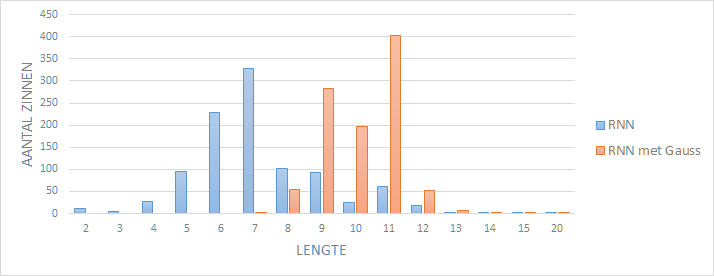
\includegraphics[width=\textwidth]{Images/gauss_length.PNG}
	\caption[Effect van gauss-normalisatie op de zinslengteverdeling]{Effect van Gauss-normalisatie op de zinslengteverdeling voor het standaard RNN-systeem.}
	\label{fig:gauss}
\end{figure}  
\begin{figure}
	\centering
	\begin{minipage}[t]{.3\textwidth}
		\centering
		\vspace{0pt}
		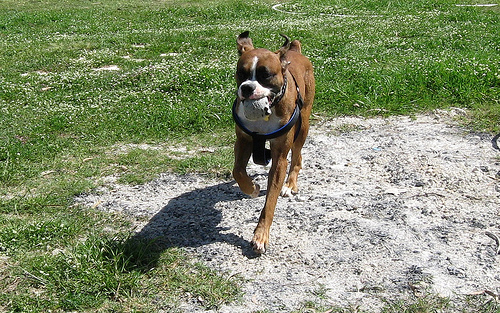
\includegraphics[width=\textwidth]{Images/Results/gauss/hond}
	\end{minipage}\hfill	
	\begin{minipage}[t]{.7\textwidth}
		\vspace{0pt}
		\begin{tabular}{ll}
			Standaard & \texttt{A dog runs through the grass} \\
			Met Gauss & \texttt{A brown and white dog is}\\
			~ & \texttt{running through the grass} \\
		\end{tabular}
	\end{minipage}
			\centering
		\begin{minipage}[t]{.3\textwidth}
			\centering
			\vspace{0pt}
			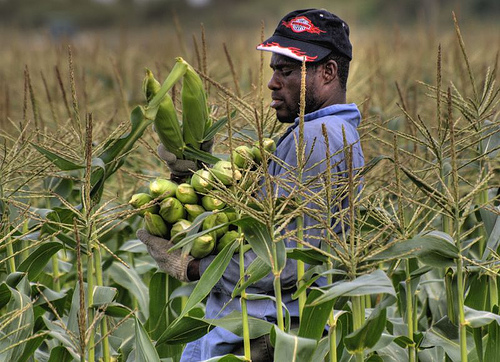
\includegraphics[width=\textwidth]{Images/Results/gauss/man}
		\end{minipage}\hfill
		\begin{minipage}[t]{.7\textwidth}
			\vspace{0pt}
			\begin{tabular}{ll}
				Standaard & \texttt{A man in a green shirt is holding a tree} \\
				Met Gauss & \texttt{A man in a blue shirt is standing }\\
				~ & \texttt{in a field} \\
			\end{tabular}
		\end{minipage}
\caption{Twee voorbeelden waar Gauss-normalisatie de gegenereerde zin verbetert.}
\label{fig:gauss_improve}
\end{figure}
\subsubsection{Min-Hinge-normalisatie}
Net als Gauss-normalisatie tracht ook Min-Hinge-normalisatie langere zinnen te genereren.
Na experimenten met hetzelfde gLSTM-netwerk met als gids CCA met een vectorgrootte van 128, blijkt dat de Min-Hinge-normalisatie hier niet in slaagt. Daarnaast verslechtert het bovendien de resultaten. Om die redenen zijn geen verdere experimenten met deze vorm van normalisatie uitgevoerd. Tabel~\ref{table:minhinge}toont de vergelijking van Gauss-normalisatie, Min-Hinge-normalisatie en geen normalisatie.

\begin{table}
	\centering
	\begin{tabular}{lllllll}
		~                  & Bleu-1 & Bleu-2 & Bleu-3 & Bleu-4 & Meteor&Zinslengte \\ \hline
		gLSTM        & 63,5   & 42,5 			& 27,9   & 18   & 15,5&7,99  \\
		gLSTM+MinHinge & 60,4   &40,4    &26,8   & 17,6   & 15,5& 7,98 \\
		gLSTM+Gauss   & 62,1   & 41,9   & 28,2   & 18,3 & 15,1& 10,54 \\ \hline
		
	\end{tabular}
	
	\caption{Automatische evaluatieresultaten voor hetzelfde gLSTM-netwerk met als gids CCA met vectorgrootte 128 en verschillende normalisatiemethodes}
	\label{table:minhinge}
\end{table}

\subsubsection{Idf-normalisatie}

\section{Vergelijking met literatuur} % (fold)
\label{sec:vergelijking_met_literatuur}
Na de grondige evaluatie van de eigen resultaten volgt in dit onderdeel een vergelijking met de resultaten uit de meest recente literatuur.
Deze vergelijking bevat onder andere het werk van Vinyals et al.~\cite{Google} dat de basis vormt voor het LSTM-netwerk in deze masterproef. 
De thesis gebruikt ook gLSTM's zoals voorgesteld in de paper van Jia et al.~\cite{Fernando2015}.
Naast deze twee hoog scorende papers bestaan er nog twee systemen die allebei aandacht integreren in hun model~\cite{Jin2015,Xu2015}.
Jin et al.~\cite{Jin2015} voegen bovendien een sc\`enevector op basis van LDA toe aan het gebruikte LSTM-netwerk.
Tabel~\ref{table:sota} biedt een overzicht van de best presterende eigen modellen in vergelijking met de beste modellen uit de literatuur.
Algemeen is duidelijk dat de best presterende modellen uit deze masterproef op de laatste paper na zeker in de buurt komen van de state-of-the-art resultaten.

De experimenten van deze masterproef werken met een aantal ongewijzigde parameters.
Deze keuze is gemaakt omdat het trainen van een netwerk met een bepaalde instelling steeds bijzonder veel tijd vraagt.
Zo duurt het trainen van een netwerk met RNN ongeveer 5 dagen op de gebruikte hardware, terwijl een netwerk met LSTM ongeveer 8 dagen vraagt.
Een betere afstelling van deze parameters maakt betere resultaten van dezelfde systemen mogelijk.
Dit is een mogelijke verklaring waarom het gLSTM-netwerk van Jia met 256 als vectorgrootte voor CCA en Gauss-normalisatie beter scoort dan onze implementatie.
Toch komen de resultaten van de masterproef zeker in de buurt.

Beide aandachtsmodellen scoren het beste in de literatuur. Het toevoegen van aandacht aan de netwerken van deze masterproef lijkt dus een veelbelovende uitbreiding.
Het model van \cite{Jin2015} claimt de hoogste resultaten op de Flickr30k testverzameling.
Het toevoegen van aandacht aan het netwerk maakt duidelijk het trainen van het netwerk complexer en bijgevolg ook trager.
Het \emph{RNN+LDA}-model doet daarom zeker niet onder. De resultaten liggen immers niet veraf en door het gebruik van een RNN en weinig complexe toevoegingen traint het sneller.
In vergelijking met ons model bestaande uit gLSTM met LDA gebruik~\cite{Jin2015} bijvoorbeeld een CNN die aparte regio's ontdekt. De ontdekte regio's en hun representatie vormen samen de voorstelling van een afbeelding in plaats van \'e\'en CNN-output zoals in deze thesis. Daarnaast maakt het gebruik van twee LSTM's met elk een andere functie. Het systeem integreert bovendien een aandachtsmodel in het netwerk.
In hun experimenten bepalen ze hun vocabularium door enkel woorden te selecteren die meer dan 20 keer voorkomen, wat hoger is dan de 5 in dit werk waardoor het systeem wel minder woorden moet leren begrijpen.
Het is opvallend dat de best scorende paper werd gepubliceerd in juni 2015, maar tot op het schrijven van deze masterproef geen publicatie heeft.

\begin{table}
	\centering
	\begin{tabular}{llllll}
		~                  & Bleu-1 & Bleu-2 & Bleu-3 & Bleu-4 & Meteor \\ \hline
		RNN+LDA            & \textbf{65,4}   & \textbf{44}     & 29,1   & 19     & 14,38  \\
		RNN+LDA+Gauss      & 62,7   & 42,6   & 28,8   & \textbf{19,5}   & 16,62  \\
		gLSTM+LDA+Gauss    & 62,7   & 42,5   & 28,8   & 19,4   & \textbf{17,4}   \\
		gLSTM+CCA          & 63,7   & 43,4   & \textbf{29,2}   & 19,3   & 15,76  \\
		gLSTM+CCA+Gauss    & 62,1   & 41,9   & 28,2   & 18,7   & 17,18  \\ \hline
		
		Google NIC~\cite{Google}           & 66,3   & 42,3   & 27,7   & 18,3   & ~      \\
		Jia (gLSTM+Gauss)~\cite{Fernando2015}  & 64,6   & 44,6   & 30,5   & 20,6   & 17,91  \\
		Jia (gLSTM+polyn.)~\cite{Fernando2015} & 59,8   & 41,3   & 29,3   & 19,2   & 18,58  \\
		Xu (Attention)~\cite{Xu2015}     & 66,9   & 43,9   & 29,6   & 19,9   & 18,46  \\
		Attention+LDA~\cite{Jin2015}      & \textbf{67}    & \textbf{47,5}   & \textbf{33}     & \textbf{24,3}   & \textbf{19,4}   \\ \hline
	\end{tabular}
	\caption{Vergelijking van de best behaalde resultaten met huidige state-of-the-art}
	\label{table:sota}
\end{table}
% section vergelijking_met_literatuur (end)

\section{Ruisgevoeligheid van CCA en LDA} % (fold)
\label{sec:ruisgevoeligheid_van_cca_en_lda_res}

% section ruisgevoeligheid_van_cca_en_lda (end)

\section{Besluit} % (fold)
\label{sec:besluit}

% section besluit (end)

